% !TEX root = 99_main.tex

% \begin{figure}
% \begin{center}
% 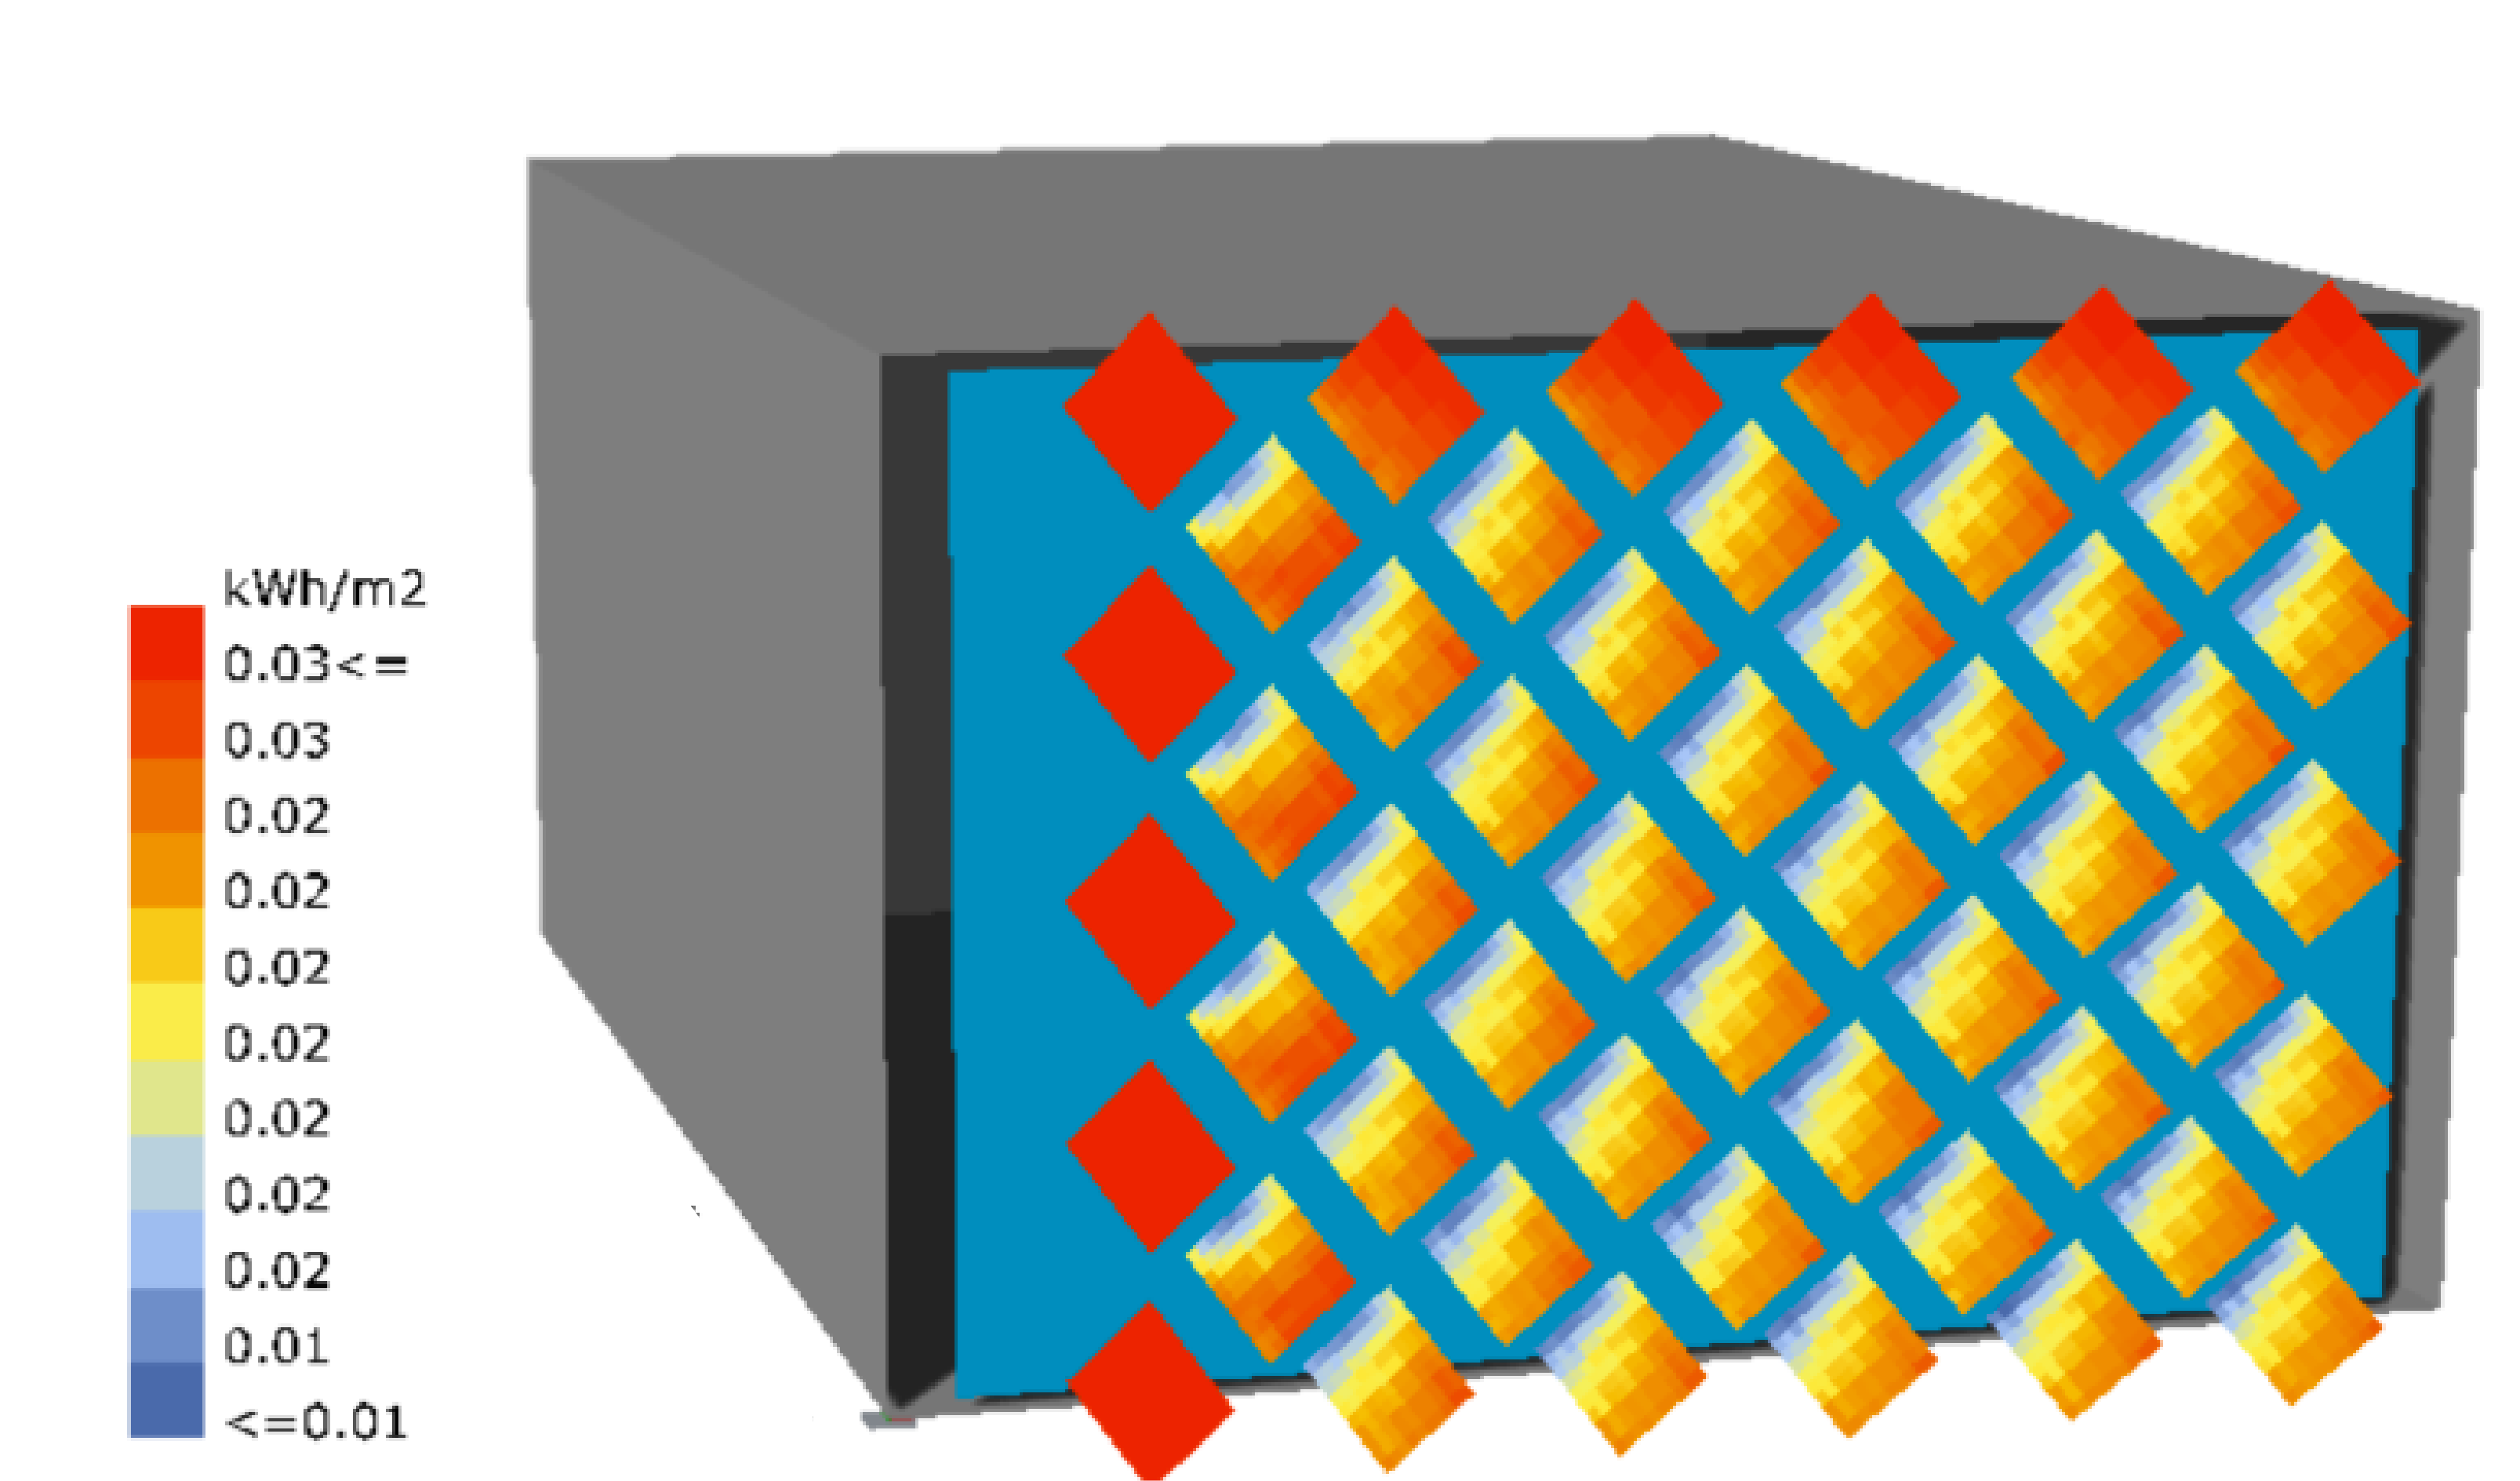
\includegraphics[width=8cm, trim= 0cm 0cm 0cm 0cm,clip]{radiationanalysis.png}
% \caption{Incident radiation on the PV panels. Light blue spots indicate areas of self shading}
% \label{fig:radiationanalysis}
% \end{center}
% \end{figure}


The optimal configurations of the ASF can be visualised using carpet-plots. Figure \ref{fig:carpetplot} details carpet-plots of the facade optimised to maximise PV generation\footnote{For this abstract, a constant efficiency of 0.1 was assumed for the PV electricity generation.}, and minimise heating, cooling and lighting demands independently. We can see how open configurations (light coloured) are chosen to minimise the building heating demands during the winter months and early mornings of spring and autumn. Likewise closed configurations (dark colours) are the preferred solutions to minimise the cooling demand during the summer months. Lighting control is only apparent during the twilight hours where the facade prefers an open position to avoid the use of artificial lighting. The PV optimisation shows to follow solar tracking for most hours and as far as the limited range of angles allows. 

\begin{figure}
\begin{center}
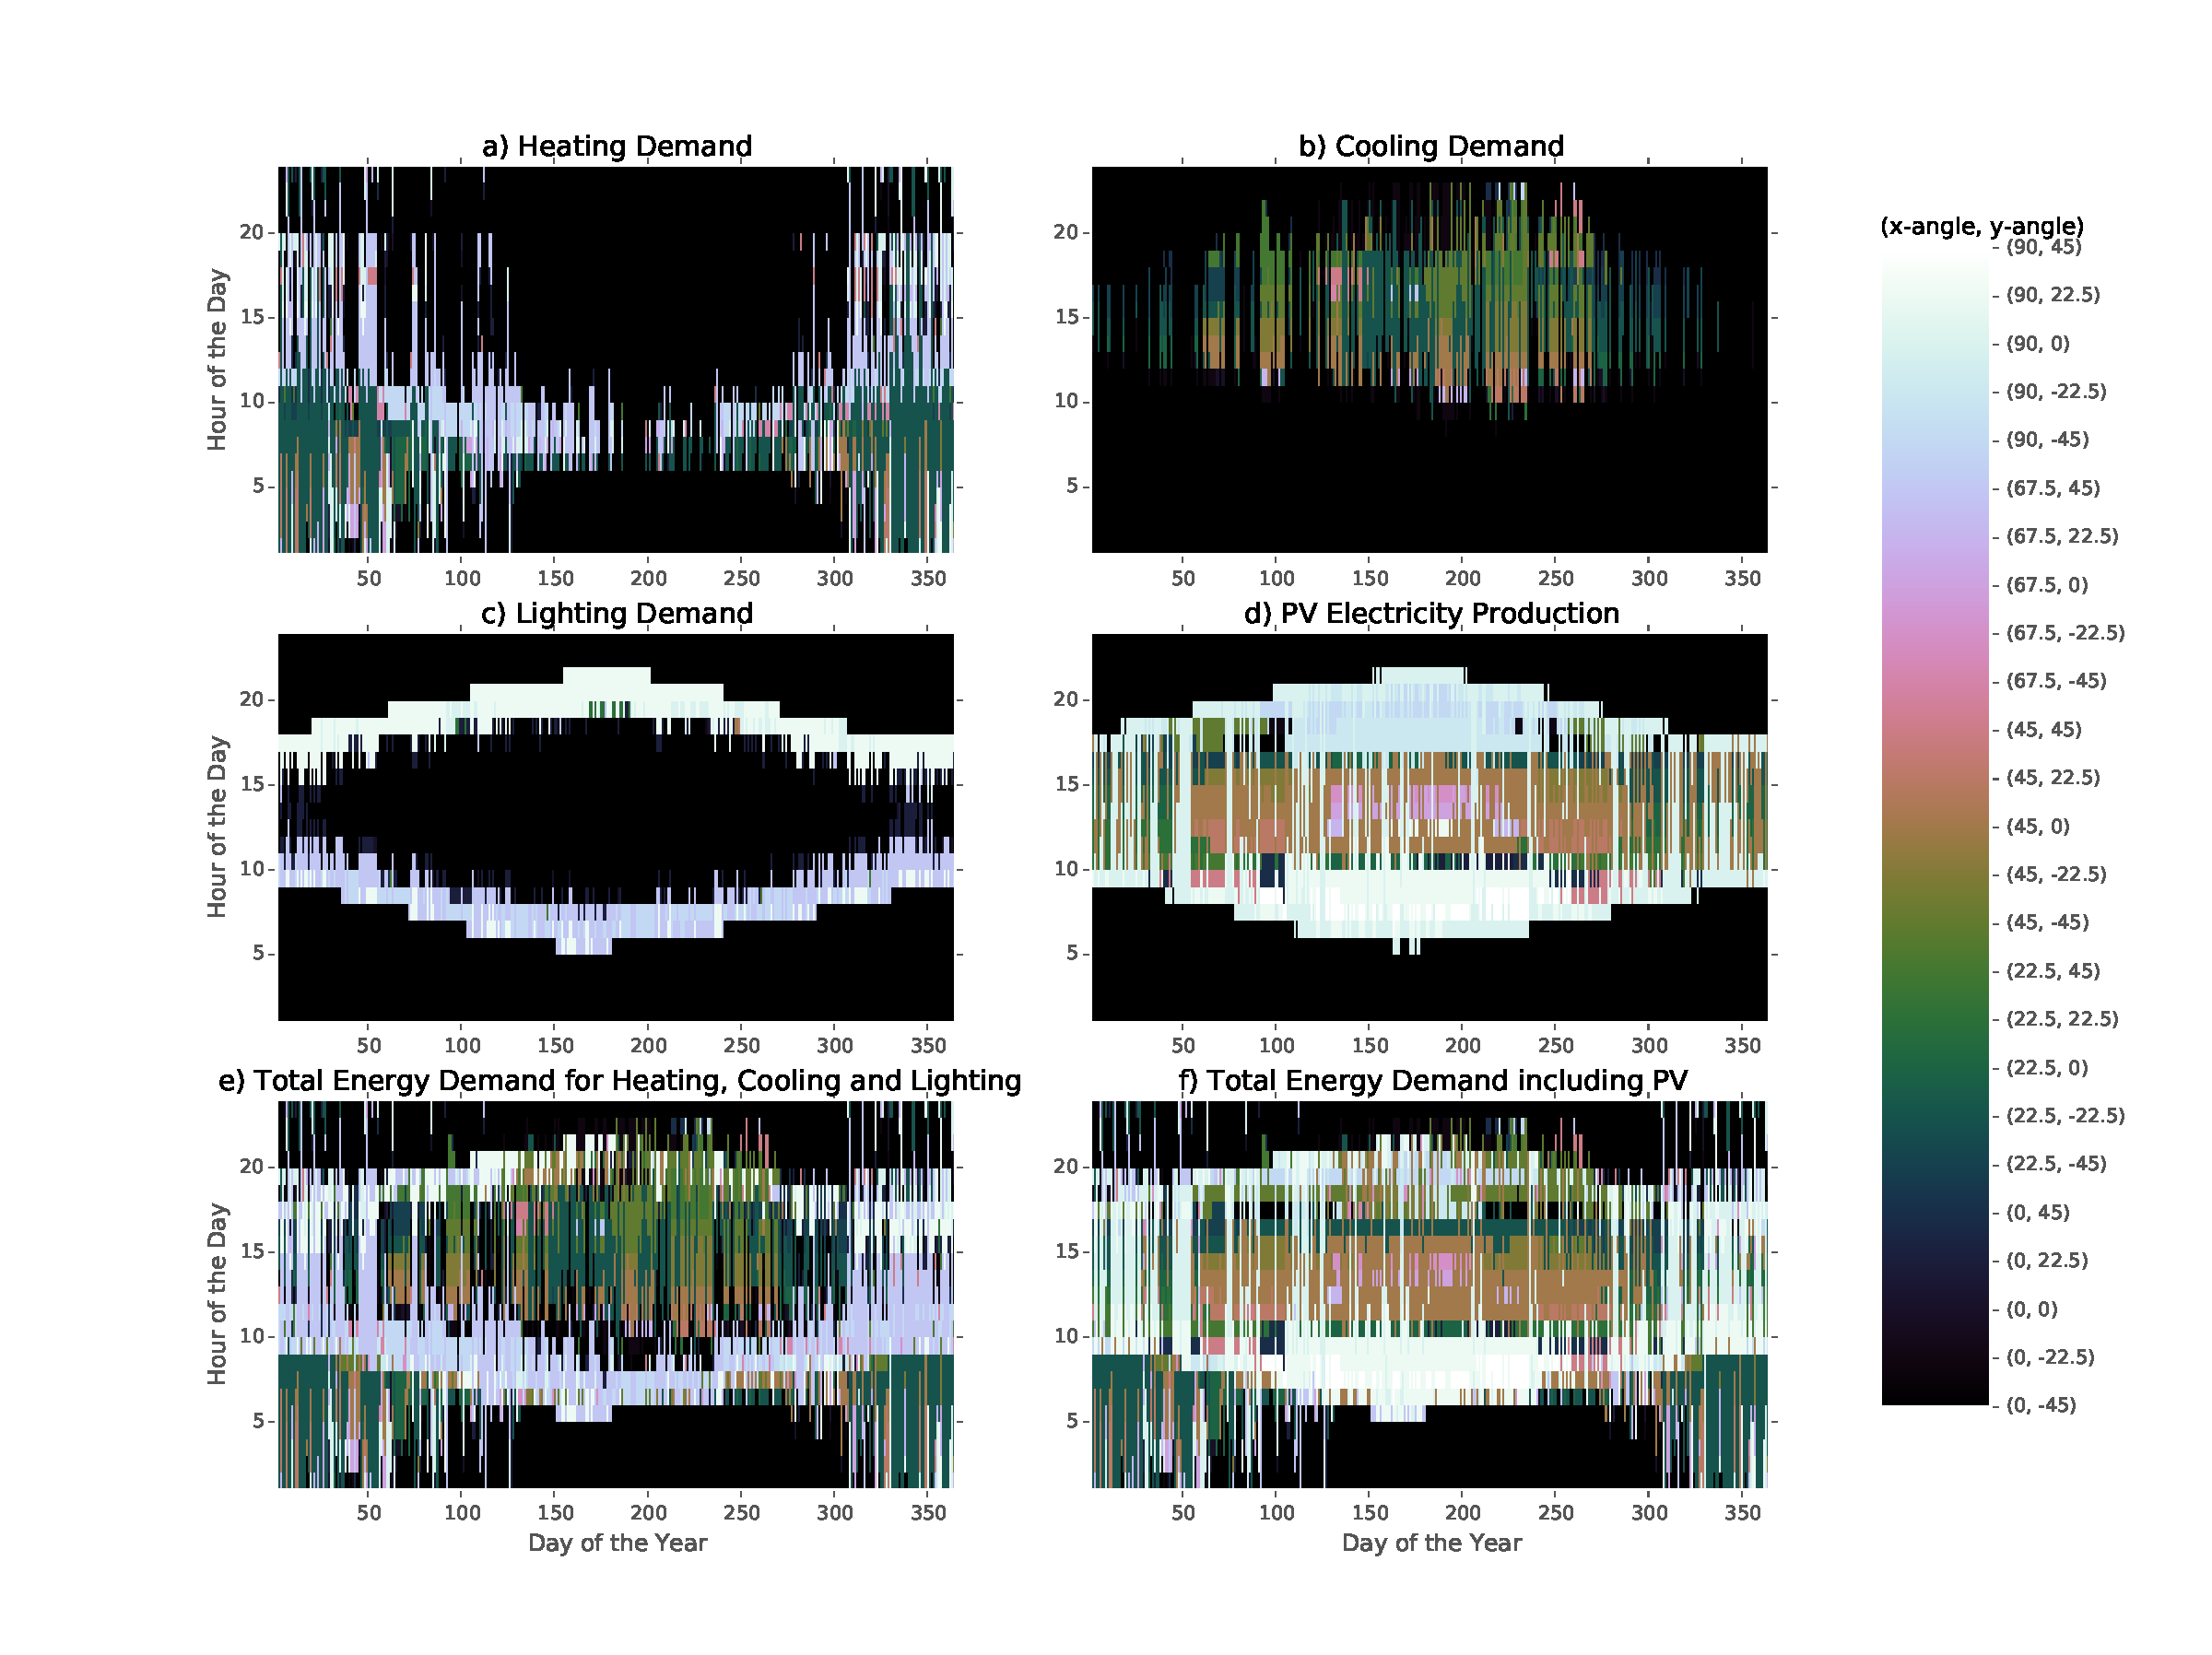
\includegraphics[width=15cm, trim= 0cm 0cm 0cm 0cm,clip]{carpet_plots.pdf}
\caption{A carpet plot detailing the optimal configuration to minimise the heating demand, cooling demand, lighting demand and maximise PV generation. Each configuration is represented by an angle of orientation around the x-axis and y-axis as seen in the legend.}
\label{fig:carpetplot}
\end{center}
\end{figure}

When the four optimisation cases are combined to achieve the configurations for total energy minimisation we get some interesting results. There is a conflict in the summer evenings between minimising lighting and cooling demands. Likewise, we also see a conflict between heating and PV production during the winter months. The overall energy optimization including PV electricity production shows a strong tendency to follow the optimal PV production pattern. 

